\subsection{Anomalous $W\gamma$ Production}
\label{sec:WgAbout_ATGC}

Most BSM physics theories predict the existence of particles which are heavier than the discovered energy range. If their masses are not accessable even by the most energetic machines, the direct detection of such particles is not possible. However, they can contribute to the productions of lower energetic particles producing loops where such heavy particles would be off-shell. This effects can be probed by precision measurements of the SM processes. In the electroweak sector processes of such interest include diboson and triboson productions which can occur through triple gauge couplings and quartic gauge couplings.\\

aTGC in MSSM and Z' from aTGC paper...\\

% EXPAND PARAGRAPH 
Constructing effective Lagrangians..\\

Triple and quartic gauge couplings (QGC) are represented by vertices with three and four bosons (Fig. \ref{fig:TGC_and_QGC_vertices}). TGC and QGC can be charged or neutral. There are variety of the SM processes where charged TGC and QGC are possible. Such processes can occur through a Feynman diagram with a vertex involving a $W$ boson and conserving charge. Corresponding vertices are $WW\gamma$, $WWZ$, $WWWW$, $WW\gamma\gamma$, $WWZ\gamma$, and $WWZZ$ (Fig. \ref{fig:TGC_and_QGC_vertices}, 1$^{st}$, 3$^{rd}$, and 5$^{th}$ diagrams). 
%REPHRASE
To search for the new physics, all these vertices are described by extended Largangian term than the SM description, involving several constants which have known values in the SM. A significant deviation of one of these constants from the known values would be an indication of a new physics.\\

As for neutral TGC and QGC, they are forbidden in the SM at the tree level but extended Lagrangian contains terms which describes neutral TGC and QGC vertices: $Z\gamma\gamma$, $ZZ\gamma$, $ZZZ$, $Z\gamma\gamma\gamma$, $ZZ\gamma\gamma$, $ZZZ\gamma$, and $ZZZZ$. Similarly to charge TGC and QGC cases, neutral TGC and QGC Largangian terms involve contants which are zero in the SM.\\  

%Maybe, general words about ATGC, where does it come from

%How it would affect the distributions and cross section

\begin{figure}[htb]
  \begin{center}
    {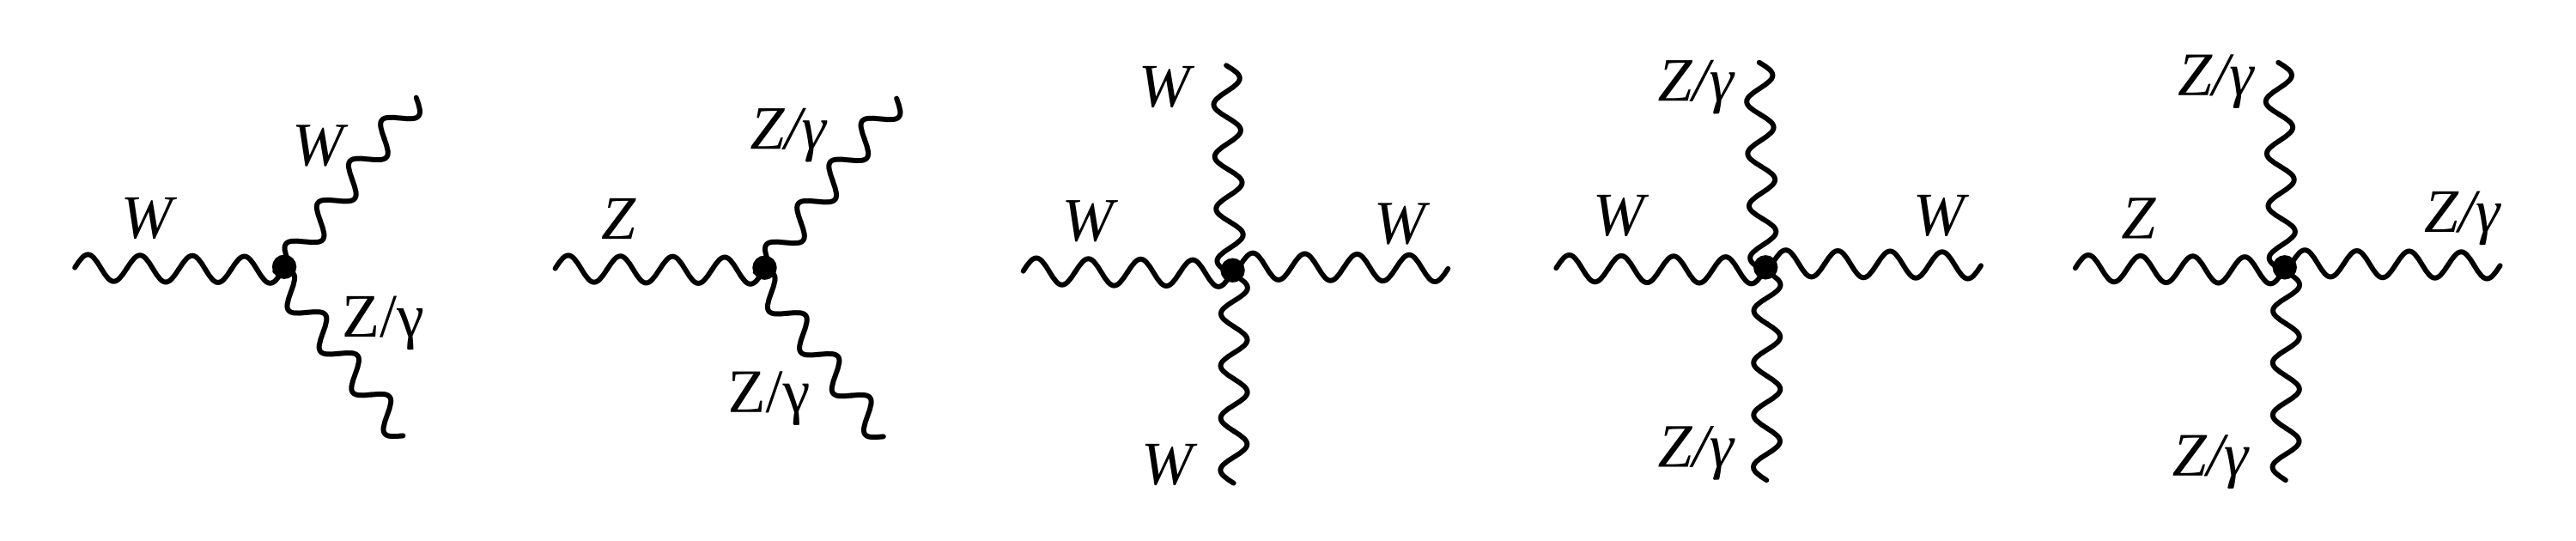
\includegraphics[width=0.95\textwidth]{../figs/WgAbout/TGC_and_QGC_vertices.png}}
    \caption{TGC and QGC vertices}
    \label{fig:TGC_and_QGC_vertices}
  \end{center}
\end{figure}


In $W\gamma$ measurement we can probe $WW\gamma$ vertex only. The most general Lorentz invariant Lagrangian of this vertex takes the following form \cite{ref_theory_aTGC}:\\

$i L_{eff}^{WW\gamma}= e [ g_1^{\gamma} A^\mu (W_{\mu\nu}^- W^{+\nu} - W_{\mu\nu}^+ W^{-\nu}) + \kappa_\gamma W_{\mu}^+ W_{\nu}^- A^{\mu\nu} + {\frac{\lambda_\gamma}{m^2_W}} A^{\mu\nu} W_\nu^{+\rho} W_{\rho\mu}^- + i g_5^\gamma \epsilon_{\mu\nu\rho\sigma}((\partial^\rho W^{-\mu})W^{+\nu} - W^{-\mu}(\partial^{\rho}W^{+\nu}))V^\sigma + i g_4^\gamma W_\mu^- W_\nu^+ (\partial^\mu A^\nu + \partial^\nu A^\mu) - \frac{\tilde{\kappa_\gamma}}{2} W_\mu^- W_\nu^+ \epsilon^{\mu\nu\rho\sigma} A_{\rho\sigma} - \frac{\tilde{\lambda_\gamma}}{2 m_W^2} W_{\rho\mu}^- W^{+\mu}_{\nu} \epsilon^{\nu\rho\alpha\beta} A_{\alpha\beta}] $\\

where $e$ is the absolute value of the electron charge, $A^\mu$ is the photon field, $W^{\pm\mu}$ are fileds of $W^\pm$ bosons, $W_{\mu\nu}=\partial_\mu W_\nu - \partial_\nu W_\mu$, $A_{\mu\nu}=\partial_\mu A_\nu - \partial_\nu A_\mu$, $m_W$ is the mass of a $W$ boson, $g_1^\gamma$, $\kappa_\gamma$, $\lambda_\gamma$, $g_5^\gamma$, $g_4^\gamma$, $\tilde{\kappa_\gamma}$, and $\tilde{\lambda_\gamma}$ are constants.\\

Despite there are 7 constants in the extended Lagrangian, only $\lambda_\gamma$ and $\kappa_\gamma$ are considered in the BSM searches. The rest of the constants are fixed to their SM values based on various considerations. Thus, $g_1^\gamma=1$ and $g_5^\gamma=0$ are fixed to obey the electromagnatic gauge invariance for the on-shell photons. The non-zero value of $g_5^\gamma$ also violates C and P conservations, and non-zero values of $g_4^\gamma$, $\tilde{\kappa_\gamma}$, $\tilde{\lambda_\gamma}$ violate the CP conservation law. Such violation parametrizations are not considered in charged TGC measurements now but might get considered in the future.\\

The presence of aTGC would have larger effects at high energy scales. Fig. \ref{fig:aTGC_Pt_Examples} shows the examples of these effects in $m_{ll}$ spectrum in 8 TeV $WW \rightarrow l\nu l\nu$ measurement (left) and $P_T^{\gamma}$ spectrum in 7 TeV $Z\gamma \rightarrow \nu\nu\gamma$ measurement (right). It is seen on the plots that aTGC spectrum at low $m_{ll}$ or low $P_T^{\gamma}$ coincides with the SM prediction but for higher $m_{ll}$ or $P_T^{\gamma}$ the disagreement becomes more significant.\\

\begin{figure}[htb]
  \begin{center}
    {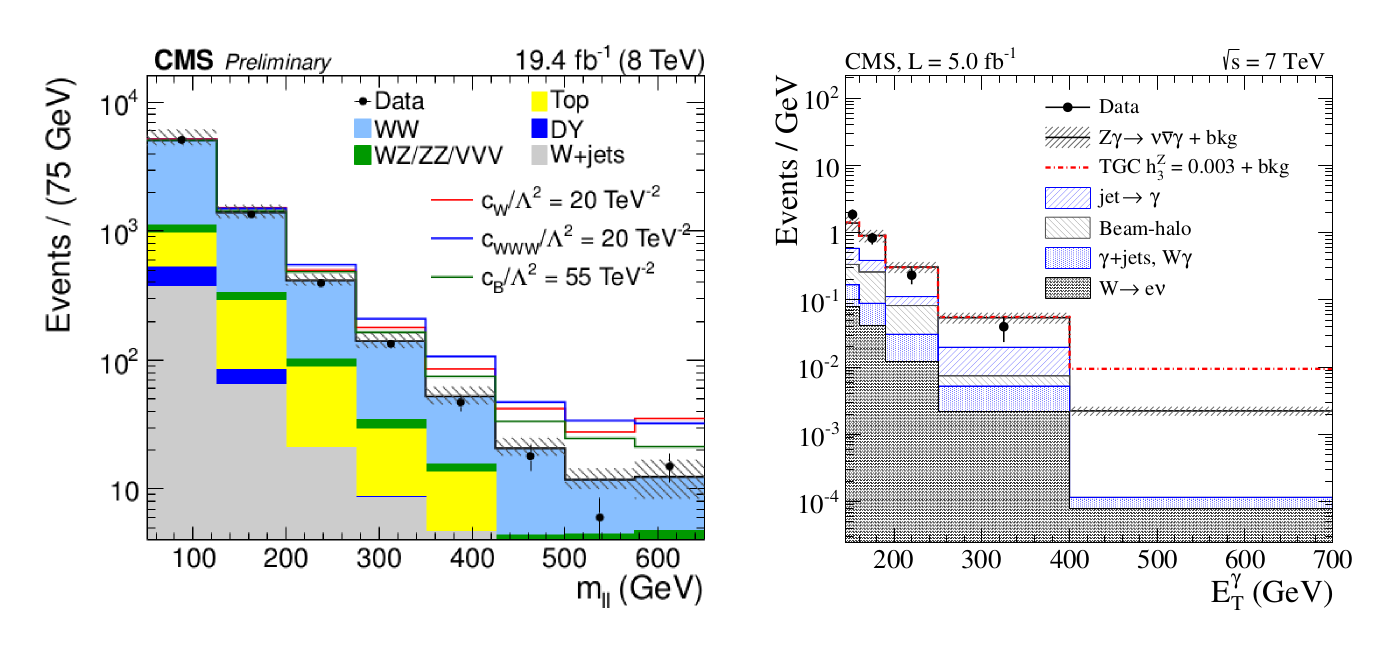
\includegraphics[width=0.85\textwidth]{../figs/WgAbout/aTGC_Pt_Examples.png}}
    \caption{Examples of the potential effects of non-zero TGC constants in $m_{ll}$ spectrum in 8 TeV $WW \rightarrow l\nu l\nu$ measurement (left) \cite{ref_CMS_8TeV_WW} and $P_T^{\gamma}$ spectrum in 7 TeV $Z\gamma \rightarrow \nu\nu\gamma$ measurement (right) \cite{ref_CMS_7TeV_Zgnunug}.}
    \label{fig:aTGC_Pt_Examples}
  \end{center}
\end{figure}

\begin{figure}[htb]
  \begin{center}
    {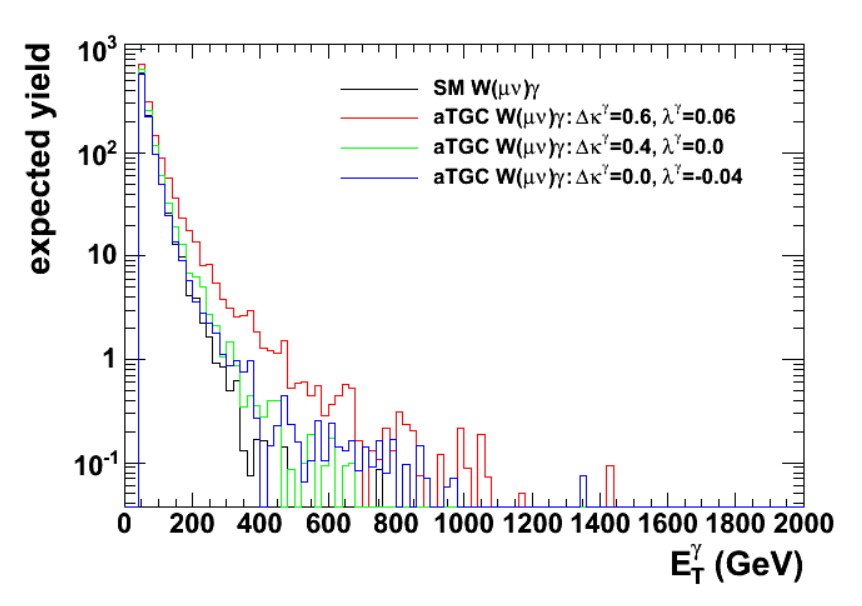
\includegraphics[width=0.85\textwidth]{../figs/WgAbout/aTGC_Pt_Wg.png}}
    \caption{Distributions of $P_T^\gamma$ of simulated $W\gamma\rightarrow\mu\nu\gamma$ events with different values of aTGC constants at LHC energy of $\sqrt{s}=7$~TeV. Source of figure:  \cite{ref_Senka_thesis}.}
    \label{fig:aTGC_Pt_Examples}
  \end{center}
\end{figure}

